Die Entwicklung des M.A.S.K.-Systems durchlief eine fundamentale Transformation – von einem komplexen Dual-Source-Ansatz hin zu einer eleganten Single-Pipeline-Lösung. Diese Evolution demonstriert, wie praktische Produktionsanforderungen zu effektiven technischen Lösungen führen können.

\subsection{Phase 1: Initiale Systemkomplexität (Januar - Februar 2025)}

\textbf{Hybrid-Tracking-Architektur:}
Basierend auf Expertenberatung entwickelte ich zunächst ein komplexes Dual-Source-System:
\begin{itemize}
    \item \textbf{MediaPipe-Integration:} ML-basierte Pose-Detection über RGB-Stream
    \item \textbf{Native Kinect-Tracking:} Hardware-Skeleton mit Tiefensensor-Daten
    \item \textbf{Kalman-Filter-Fusion:} Synchronisation und Glättung beider Datenquellen
    \item \textbf{Adaptive Fallback-Logik:} Automatische Umschaltung bei Tracking-Verlust
\end{itemize}

\begin{algorithm}[H]
\caption{Ursprüngliche Dual-Source-Verarbeitungsschleife}
\begin{algorithmic}[1]
    \State $\text{kinect\_data} \leftarrow \text{receiveKinectSkeleton()}$
    \State $\text{mediapipe\_data} \leftarrow \text{processRGBStream()}$
    \If{$\text{mediapipe\_data} \neq \text{null} \land \text{kinect\_data} \neq \text{null}$}
        \State $\text{skeleton} \leftarrow \text{fusionProcess}(\text{kinect\_data}, \text{mediapipe\_data})$
    \Else
        \State $\text{skeleton} \leftarrow \text{fallbackToStrongerSource()}$
    \EndIf
    \State $\text{skeleton} \leftarrow \text{applyKalmanFilter}(\text{skeleton})$
    \State \textbf{evaluateTriggers}(\text{skeleton})
\end{algorithmic}
\end{algorithm}

\textbf{Erste Validierung:}
Komparative Tests zwischen MediaPipe und Kinect zeigten MediaPipes bessere Robustheit bei partieller Okklusion. Das ML-Modell generierte höhere Confidence-Werte für nicht-sichtbare Körperregionen, was für komplexe Choreographien entscheidend war.

\subsection{Phase 2: Visual Requirements Engineering (März 2025)}

\textbf{Stakeholder-Driven Design:}
Die intensive Zusammenarbeit mit den Filmakademie-Designerinnen führte zu präzisen Visual-Anforderungen, die über einfache Bewegungstrigger hinausgingen:

\begin{itemize}
    \item \textbf{Adaptive Größenmodulation:} Visuals skalieren basierend auf Performer-Zustand
    \item \textbf{Räumliche Choreographie:} Präzise Beamer-Projektion um Performer herum
    \item \textbf{Emotionale Responsivität:} Visual-Transformation entsprechend choreographischer Intentionen
\end{itemize}

\begin{figure}[H]
    \centering
    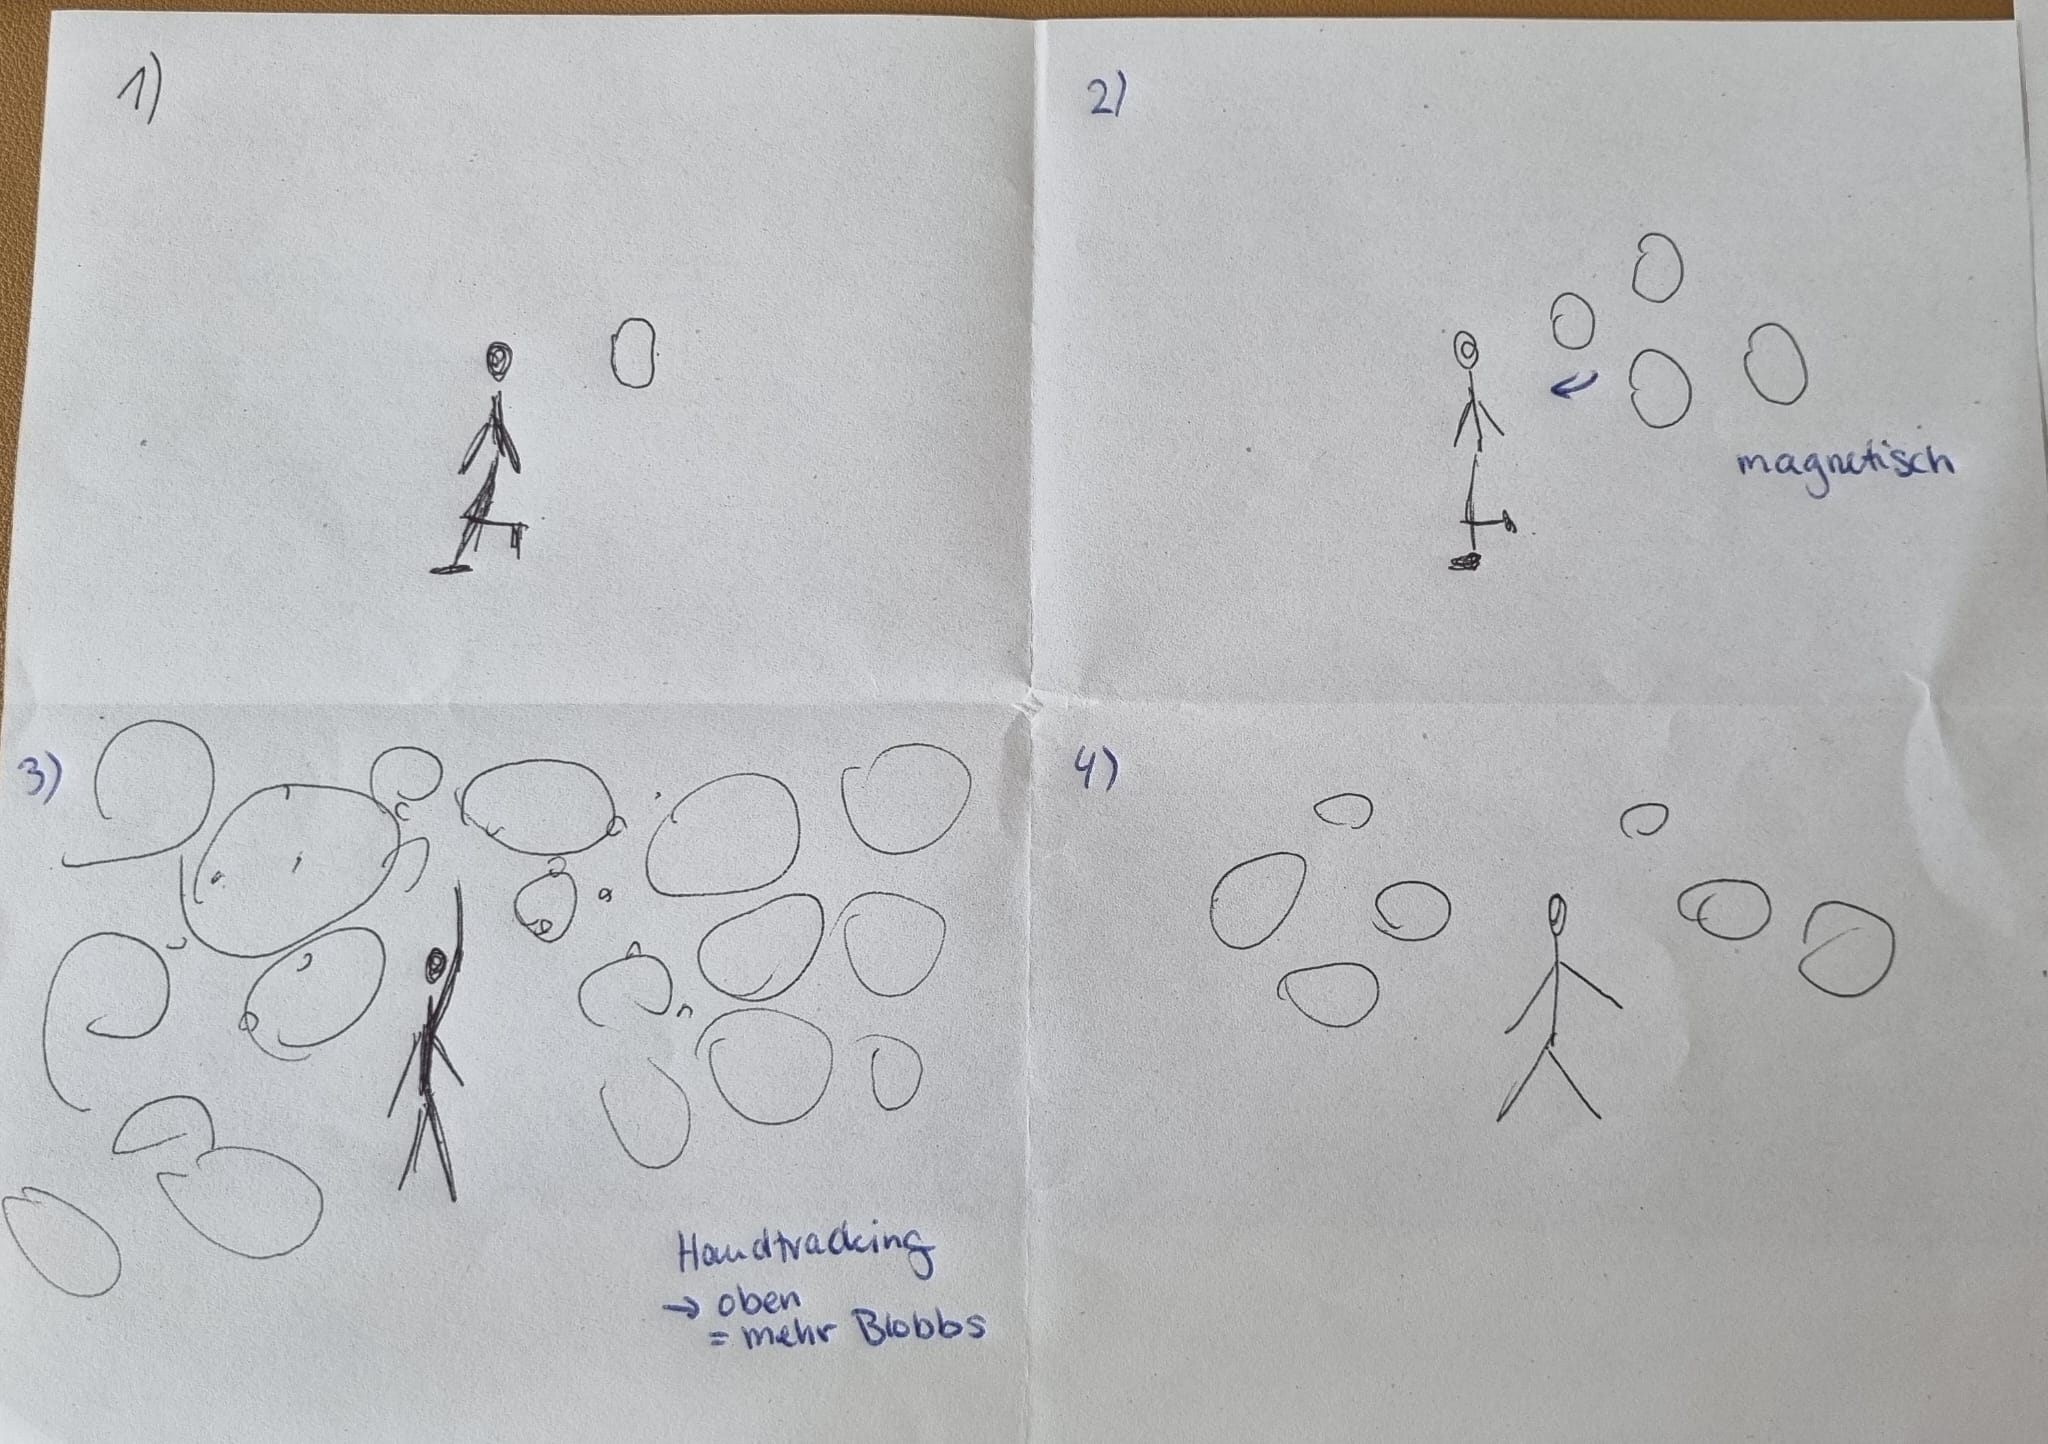
\includegraphics[width=0.8\textwidth]{images/Sprint3_1.jpg}
    \caption{Designkonzept: Skalierungsresponsive Visual-Transformation}
    \label{fig:design_evolution}
\end{figure}

\textbf{Technische Herausforderungen:}
Diese künstlerischen Anforderungen stellten das ursprüngliche System vor erhebliche Performance-Probleme. Die Dual-Source-Architektur erwies sich als zu ressourcenintensiv für komplexe Real-time-Visuals.

\newpage

\subsection{Phase 3: Architektonische Vereinfachung (April 2025)}

\textbf{Strategische Entscheidung:}
Angesichts der Performance-Limitationen entschied ich mich für eine radikale Vereinfachung: Vollständige Fokussierung auf MediaPipe als primäres Tracking-System.

\textbf{Systemvereinfachung:}
\begin{itemize}
    \item \textbf{Kinect-Elimination:} Entfernung der nativen Kinect-SDK-Abhängigkeiten
    \item \textbf{MediaPipe-Optimierung:} Direkter RGB-zu-Pose-Pipeline ohne Datenfusion
    \item \textbf{Modulare Architektur:} Plug-and-Play TouchDesigner-Container
    \item \textbf{Performance-Boost:} CPU-Nutzung reduziert
\end{itemize}

\textbf{Unerwartete Erkenntnisse:}
Die Vereinfachung führte nicht nur zu besserer Performance, sondern auch zu erhöhter Systemstabilität und einfacherer Wartung – ein klassisches Beispiel für „weniger ist mehr" in der Systemarchitektur.

\subsection{Phase 4: Produktionsvalidierung und Lösungsfindung (Mai 2025)}

\textbf{Beleuchtungsproblem:}
Bei den ersten Produktionstests stellte sich heraus, dass intensive Beamer-Projektionen die RGB-Kameras überlasten und MediaPipe funktionsunfähig machen. Ein fundamentales Problem für Live-Performance-Anwendungen.

\textbf{Praxisorientierte Lösung - Infrarot-Pipeline:}
Unter Produktionsdruck entwickelte ich eine spezifische Adaptation: Routing des Kinect-Infrarot-Streams (512×424 Pixel, 16-bit) über OBS Virtual Camera direkt zu MediaPipe.

\begin{figure}[H]
    \centering
    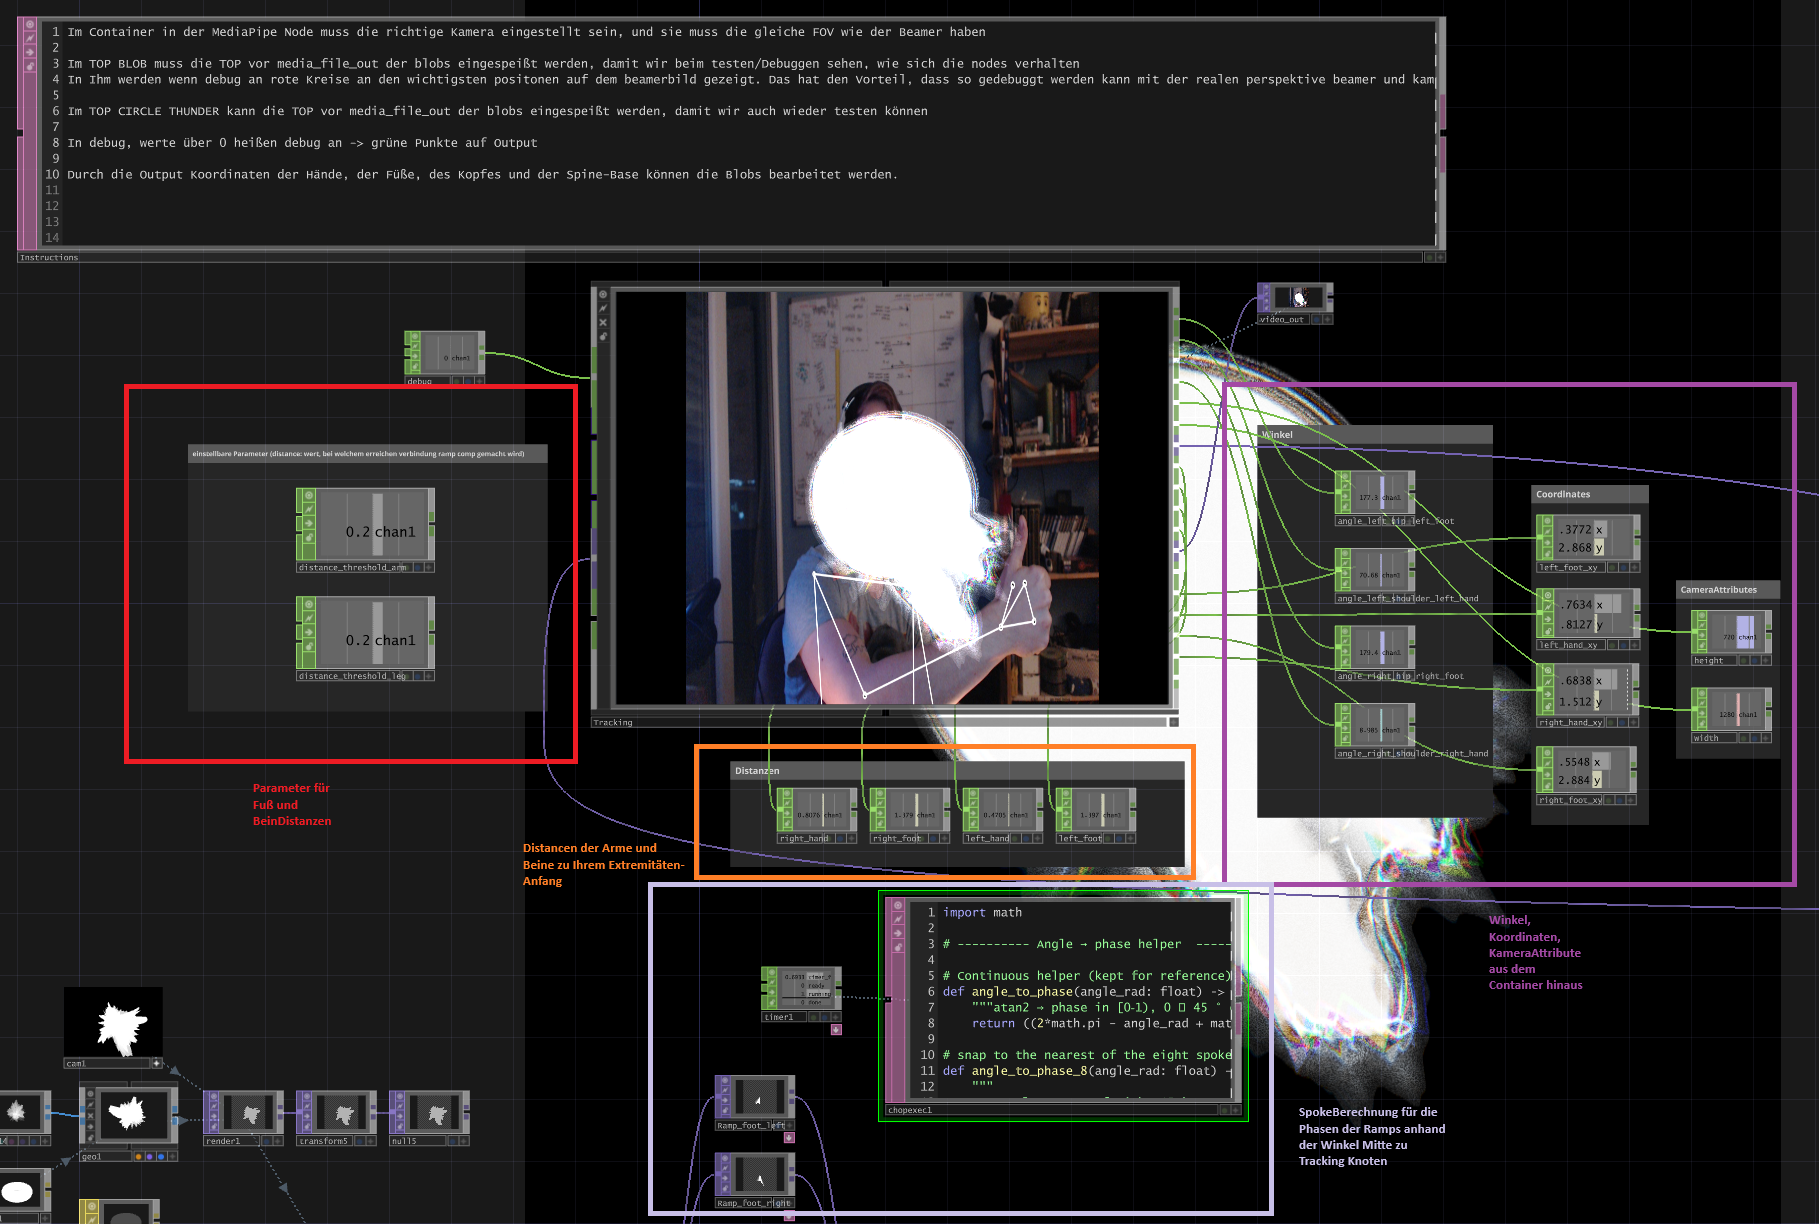
\includegraphics[width=0.9\textwidth]{images/docupictures/TopDown_KreisZuRampsParametisierteBerechnungen.png}
    \caption{Infrarot-MediaPipe-Pipeline: Technische Lösung für Produktionsumgebungen}
    \label{fig:infrared_solution}
\end{figure}

\textbf{Technische Spezifikationen der finalen Lösung:}
\begin{itemize}
    \item \textbf{Input:} Kinect V2 Infrarot-Stream (512×424@30fps)
    \item \textbf{Processing:} OBS Virtual Camera → MediaPipe Pose Detection
    \item \textbf{Output:} TouchDesigner-kompatible Koordinaten-CHOPs
\end{itemize}

\subsection{Phase 5: Spezialisierte Visual-Systeme}

\textbf{Drei finale Implementierungen:}

\textit{1. Hand-Feuer-Effekte:}
ParticleGPU-basierte blaue Flammenpartikel, die Handbewegungen in Echtzeit folgen. Implementation extrahiert Hand-Landmarks (MediaPipe Nodes 15/16) und transformiert diese in normalisierte Bildschirmkoordinaten.
Dafür werden per Script die Hand-Node-Positionen in TouchDesigner als Partikel-Emitter genutzt. Die Partikel haben eine Lebenszeit von 1,2 Sekunden und werden basierend auf der Handgeschwindigkeit emittiert.


\textit{2. Adaptive Kopfpartikel:}
Zustandsbasiertes System mit Hand-zu-Schulter-Positionsvergleich. Eine Interpolationsfunktion sorgt für sanfte Übergänge zwischen zwei visuellen Modi.
Die Visuals folgen der Kopf-Node über Setzung des particleGPU offsets von der Mitte des Bildschirms per Script-Mapping.

\textit{3. 64-Spike Radialsystem:}
Hochpräzise Winkelauflösung (5,625°) für Extremitätenerkennung. Polar-Koordinaten-Mapping ermöglicht exakte Richtungstrigger basierend auf Körperhaltung.
Per Skript werden die Hand- und Fußpositionen relativ zum Bildschirmzentrum in Polarkoordinaten umgerechnet. Der atan2-Algorithmus mappt Winkel auf diskrete Spike-Indizes (0-63),
und wird anschließend auf RAMP positionen gemappt, und per connect- disconnect logic anhand der Distanz der Nodes zur Mitte zum Comp verbunden.

\newpage

\subsection{Technische Bilanz}

\textbf{Entwicklungsevolution im Überblick:}
\begin{table}[H]
    \centering
    \begin{tabular}{|l|c|c|c|}
        \hline
        \textbf{Metrik} & \textbf{Initial (Dual-Source)} & \textbf{Vereinfacht (MediaPipe)} & \textbf{Final (IR-Pipeline)} \\ \hline
        CPU-Nutzung & Hoch & Gering & Etwas Mehr als Vereinfacht\\ \hline
        Tracking-Präzision & 75\% & 70\% (RGB) & 90\% (IR) \\ \hline
        Setup-Zeit & 45 Minuten & 15 Minuten & 20 Minuten \\ \hline
        Systemkomplexität & Hoch & Niedrig & Mittel \\ \hline
        Produktionstauglichkeit & Nein & Bedingt (da RGB überbelichtbar) & Ja \\ \hline
    \end{tabular}
    \caption{Systemevolution: Technische Verbesserungen über Entwicklungsphasen (Estimates ohne professionelle Messung!)}
    \label{tab:system_evolution}
\end{table}

\textbf{Lessons Learned:}
\begin{itemize}
    \item \textbf{Constraints fördern Lösungsansätze:} Die Beleuchtungsbeschränkung führte zur infrarot-basierten Adaptation
    \item \textbf{Systemvereinfachung verbessert Robustheit:} MediaPipe-only erwies sich als stabiler als Dual-Source-Ansatz
    \item \textbf{Produktionsvalidierung ist entscheidend:} Reale Umgebungsbedingungen deckten wichtige Designanpassungen auf
    \item \textbf{Interdisziplinarität steigert Qualität:} Zusammenarbeit mit Designerinnen optimierte sowohl technische als auch künstlerische Aspekte
\end{itemize}

Die Entwicklung von M.A.S.K. demonstriert, wie iterative Vereinfachung und praxisorientierte Problemlösung zu eleganten, produktionstauglichen Lösungen führen können. Das finale System ist nicht nur technisch ausgereift, sondern auch konzeptuell klarer und wartungsfreundlicher als die ursprüngliche komplexe Architektur.